\documentclass[12pt]{article}
\usepackage{mathematics}

\begin{document}

\title{Oxford M2 - Real Analysis II - Continuity and Differentiability
  \footnotetext{\url{https://courses.maths.ox.ac.uk/node/37497}}} \author{Dan Davison}
\author{}
\date{}
\maketitle

\section{Sheet 2}

\begin{mdframed}
  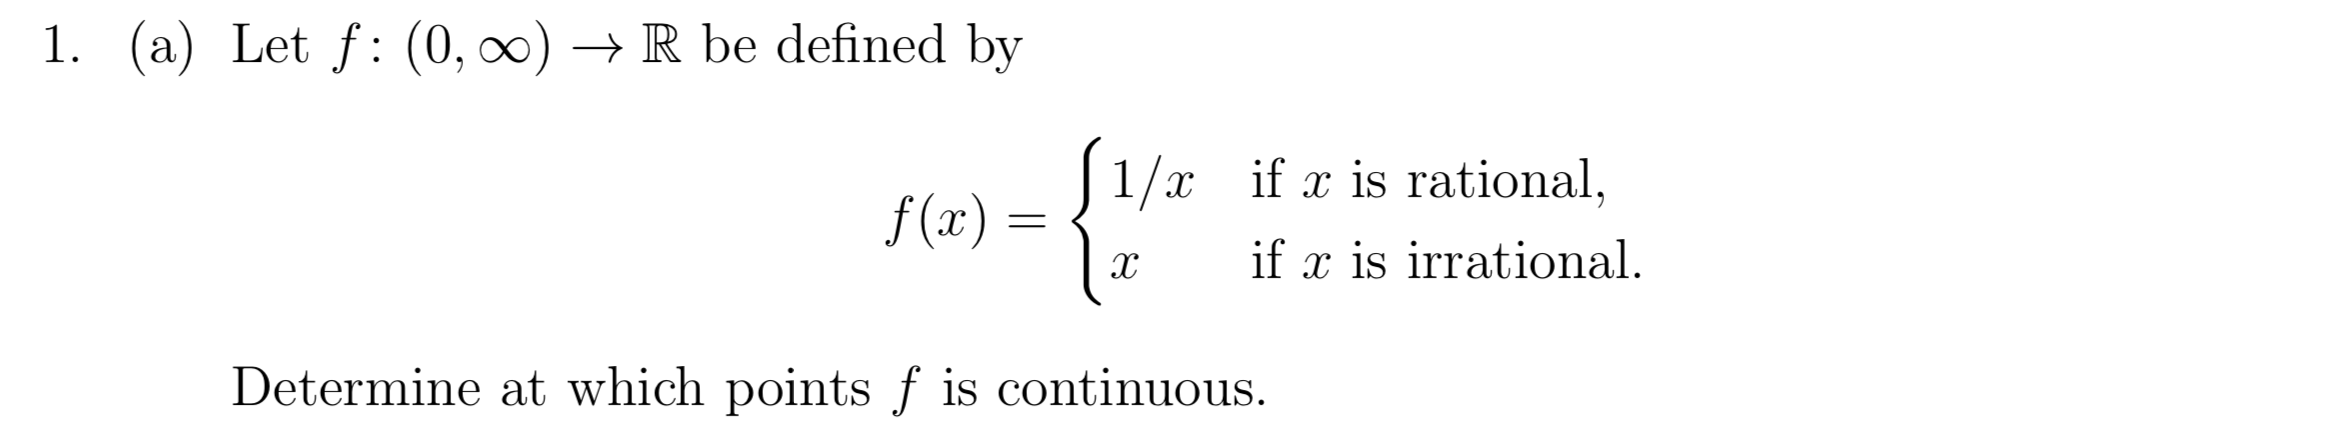
\includegraphics[width=400pt]{img/oxford-prelims-M2-analysis-II-sheet-2-1a.png}
\end{mdframed}

\begin{theorem*}
  $f$ is continuous at 1 and -1 only.
\end{theorem*}

\begin{proof} Let $q \in \Q \cap (0, \infty)$.

  Note that there exists a sequence $(q_n)$ such that $q_n \in \Q$, $q_n \neq q$ and
  $\LimEq{q_n}{q}{n}{\infty}$.

  From Theorem 1.13 (Algebra of Limits) we have $\Lim{x^\1}{x}{q} = q^\1$.

  Therefore from Theorem 1.10 we have

  % Therefore $\LimEq{f(q_n)}{1/q}{n}{\infty}$.

  Also, there exists a sequence $(p_n)$ such that $p_n \in \R\setminus\Q$, and
  $\LimEq{p_n}{q}{n}{\infty}$.


\end{proof}

\begin{definition*}[continuity]
  $f$ is continuous at $a$ if $\LimEq{f(x)}{f(a)}{x}{a}$.
\end{definition*}

\begin{definition*}[limit]
  $\LimEq{f(x)}{f(a)}{x}{a}$ if for all $\epsilon > 0$ there exists $\delta > 0$ such that
  $0 < |x - a| < \delta \implies |f(x) - f(a)| < \epsilon$.
\end{definition*}

\begin{theorem*}
  $f$ is continuous nowhere. I.e. for all $a \in (0, \infty)$ there exists $\epsilon > 0$ such that
  for all $\delta > 0$ there exists $x \in (0, \infty)$ such that $|x - a| < \delta$ and yet
  $|f(x) - f(a)| \geq \epsilon$.
\end{theorem*}

\begin{intuition*}
  However small we make $\delta$, an interval of radius $\delta$ centered at a rational point will
  contain irrational points, and vice versa.
\end{intuition*}

\begin{proof}~\\
  Let $x \in (0, \infty)$.

  Let $q \in \Q \cap (0, \infty)$. Then there exists a sequence:




  Fix $\delta > 0$. Note that there are both rational $x$ and
  irrational $x$ satisfying $0 < |x - q| < \delta$. Therefore the maximum value attained by
  $|f(x) - f(q)|$ is $||$
\end{proof}



Let $p \in (0, \infty) \setminus \Q$ be an

Let $p, q \in (0, \infty)$ with $p \notin \Q$ and $q \in \Q$.

\end{document}